\chapter{Experimental Results}
\pagestyle{fancy}\lhead{\textbf \footnotesize\it{Experimental Results}}
\pagestyle{fancy}\chead{} \pagestyle{fancy}\rhead{}
\pagestyle{fancy}\lfoot{\textbf {\small\it{Univ-Mascara/Computer Science: 2025}}} 
\pagestyle{fancy}\cfoot{} \pagestyle{fancy}\rfoot{\thepage}
%%%%%%%%%%%%%%%%%%%%%%%%%%%%%%%%%%%%%%%%
\section{Introduction}\label{start6}
In this chapter, we present the experimental results of applying our novel algorithm to SASRec and compare its performance with SASRec tested using MOL. The goal of these experiments is to assess the effectiveness of our approach in improving recommendation accuracy, model efficiency, and overall performance metrics.


\section{Experimental Results}\label{sec3}
In order to measure the effectiveness of our proposed method, we perform a comprehensive evaluation of both the retrieval algorithm and the Mixture-of-Logits (MoL) approach. This assessment focuses on the next-item prediction task, a fundamental challenge in recommendation systems\cite{kang2018selfat},
where the goal is to predict the most relevant item a user will interact with next based on their past interactions. 
\subsection{Dataset}
We conducted experiments using two MovieLens datasets : ML-100K and ML-1M \cite{Harper2015}which are widely used benchmarks for evaluating sequential recommendation models as detailed in Table\ref{tab_movielens}.\\
\begin{table}[h]
	\centering
	\renewcommand{\arraystretch}{1.2}
	\begin{tabular}{|l|p{10cm}|}
		\hline
		\textbf{Dataset} & \textbf{Description} \\
		\hline
		\textbf{MovieLens-100K} & 100,000 ratings (1-5 scale) from 943 users on 1,682 movies. \\
		& Each user has rated at least 20 movies. \\
		& Includes user demographic information (age, gender, occupation, zip code). \\
		\hline
		\textbf{MovieLens-1M} & 1,000,209 ratings from 6,040 users on approximately 3,900 movies. \\
		& Data collected from users who joined MovieLens in 2000. \\
		& Represents a larger-scale recommendation scenario. \\
		\hline
	\end{tabular}
	\caption{Summary of MovieLens datasets}
	\label{tab_movielens}
\end{table}

\subsection{ Setup }For both datasets, We utilize the SASRec architecture as our sequential user encoder, a model renowned for achieving state-of-the-art performance in next-item prediction tasks. This architecture processes the user's historical interaction sequence, generating embeddings that encapsulate the user's preferences at each time step. These embeddings serve as the foundation for predicting the next item in the sequence.

The query \( q \) represents the user's state at a specific time step, derived from their interaction history. In the MoL (Mixture of Logits) framework,\( q \)is transformed into \( Pq \)
embeddings through a multi-layer perceptron (MLP).
\subsection{Impact of Hyperparameters}
For fair comparison, we maintained consistent architectural choices and training conditions across all experiments, We conducted an extensive hyperparameter analysis comparing both approaches (Hybrid+SAS and MoL+SAS) across different architectural configurations. All experiments were Implemented in TensorFlow and trained on a Google Colab environment with a T4 GPU. We use the Adam optimizer with a learning rate of 0.001. For the hybrid algorithm, we initialize the threshold (Tinit) to 0.3 and adaptively adjust it during training. We discuss detailed hyperparameter settings in table \ref{tab:100k_movies}, table \ref{tab:1m_movies}


\newpage


\setlength{\tabcolsep}{1pt} % Increase column padding

\begin{table}[h]
	\centering
	\large
	\renewcommand{\arraystretch}{1.7} % Increase row spacing
	\resizebox{\textwidth}{!}{  % Scale table to fit width
		\begin{tabular}{|l|c|c|c|c|c|c|c|c|}
			\hline
			\textbf{Model} & \textbf{\shortstack{Max \\ Sequence Length}} & 
			\textbf{\shortstack{Embedding \\ Dimension}} & 
			\textbf{\shortstack{Number \\ of Heads}} & 
			\textbf{\shortstack{Feedforward \\ Dimension}} & 
			\textbf{\shortstack{Batch \\ Size}} & 
			\textbf{Epochs} & 
			\textbf{\shortstack{Val \\ Loss}} & 
			\textbf{\shortstack{Val \\ Accuracy}} \\
			\hline
			Hybrid+SAS & 50  & 128  & 2 & 128  & 128 & 12 & 5.3036 & 0.1584  \\ \hline
			MoL+SAS    & 50  & 128  & 2 & 128  & 128 & 12 & 5.3152 & 0.1582  \\ \hline
			Hybrid+SAS & 128 & 256  & 4 & 256  & 128 & 10 & 3.6364 & 0.4301  \\ \hline
			MoL+SAS    & 128 & 256  & 4 & 256  & 128 & 10 & 3.6374 & 0.4299 \\\hline
			Hybrid+SAS & 512 & 512  & 4 & 512  & 128 & 10 & 1.2808 & 0.8120 \\ \hline
			MoL+SAS    & 512 & 512  & 4 & 512  & 128 & 10 & 1.3050 & 0.8016 \\\hline
		\end{tabular}
	}
	\caption{Results on 100kMovies dataset}
	\label{tab:100k_movies}
\end{table}
\setlength{\tabcolsep}{1pt} % Increase column padding
\begin{table}[h]
	\centering
	\large
	\renewcommand{\arraystretch}{1.7} % Increase row spacing
	\resizebox{\textwidth}{!}{  % Scale table to fit width
		\begin{tabular}{|l|c|c|c|c|c|c|c|c|}
			\hline
			\textbf{Model} & \textbf{\shortstack{Max \\ Sequence Length}} & 
			\textbf{\shortstack{Embedding \\ Dimension}} & 
			\textbf{\shortstack{Number \\ of Heads}} & 
			\textbf{\shortstack{Feedforward \\ Dimension}} & 
			\textbf{\shortstack{Batch \\ Size}} & 
			\textbf{Epochs} & 
			\textbf{\shortstack{Val \\ Loss}} & 
			\textbf{\shortstack{Val \\ Accuracy}} \\
			\hline
			Hybrid+SAS & 50  & 128  & 2 & 128  & 128 & 10 & 4.5721 & 0.1530  \\ \hline
			MoL+SAS    & 50  & 128  & 2 & 128  & 128 & 10 & 4.5733 & 0.1526  \\ \hline
			Hybrid+SAS & 128 & 256  & 4 & 256  & 128 & 10 & 3.4152 & 0.3680  \\ \hline
			MoL+SAS    & 128 & 256  & 4 & 256  & 128 & 10 & 3.4671 & 0.3627  \\ \hline
			Hybrid+SAS & 512 & 512  & 4 & 512  & 128 & 10 & 1.0275 & 0.8350  \\ \hline
			MoL+SAS    & 512 & 512  & 4 & 512  & 128 & 10 & 1.0350 & 0.8276  \\ \hline
			
		\end{tabular}
	}
	\caption{Results on 1M Movies dataset}
	\label{tab:1m_movies}
\end{table}
Both approaches demonstrate significant performance improvements as model capacity increases, with larger configurations consistently delivering better results. For instance, when increasing the model's capacity such as expanding the (Max Sequence Length: 512, Embedding Dimension: 512, Number of Heads: 4, Feed-Forward Dimension: 512) the hybrid algorithm combined with SASRec (Hybrid+SAS) achieves notable gains, particularly in the most resource-intensive setup. On the ML-100K dataset, Hybrid+SAS reaches a score of\textbf{0.8120} compared to the baseline's \textbf{0.8016}, while on ML-1M, it achieves \textbf{0.8350} versus \textbf{0.8276} The ML-1M dataset generally benefits more from increased capacity, with the performance gap between datasets narrowing as the model scales. While smaller configurations provide a balance of efficiency and performance, the largest configuration, despite its higher computational demands, yields the best results, making it suitable for scenarios where resources are not a constraint. Both approaches show similar benefits from scaling, but Hybrid+SAS maintains a consistent edge in performance.


\subsection {Impact of Adaptive k-Variations on Model Performance}
As shown in Figures~\ref{fig:k_changes_100K} and \ref{fig:k_changes_1M}, the value of $k$ fluctuates across epochs for both MovieLens 100K and MovieLens 1M datasets. These variations indicate the adaptive nature of $k$ in response to the dataset characteristics and training progress. In the following section, we analyze how these changes influence model performance.  

\begin{figure}[htbp]
	\centering
	\begin{subfigure}{0.48\textwidth}
		\centering
		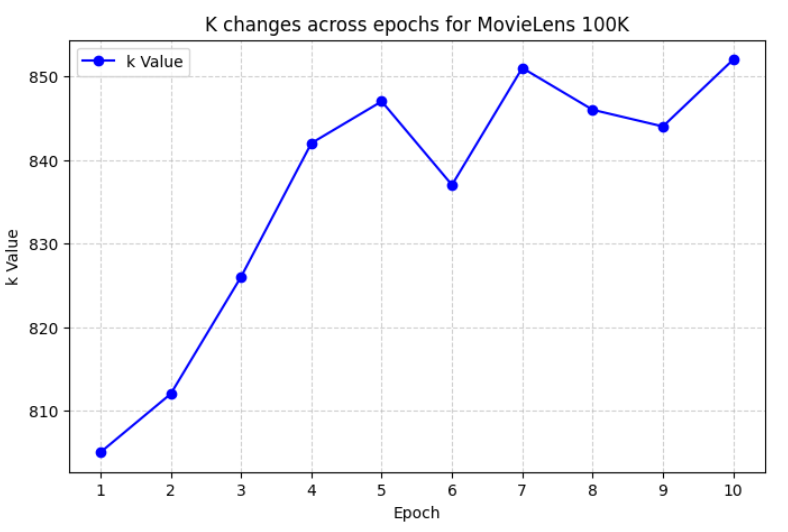
\includegraphics[width=\linewidth]{Figures/CHAGES_OF_K_FOR_100k.png}
		\caption{K changes across epochs for MovieLens 100K}
		\label{fig:k_changes_100K}
	\end{subfigure}
	\hfill
	\begin{subfigure}{0.48\textwidth}
		\centering
		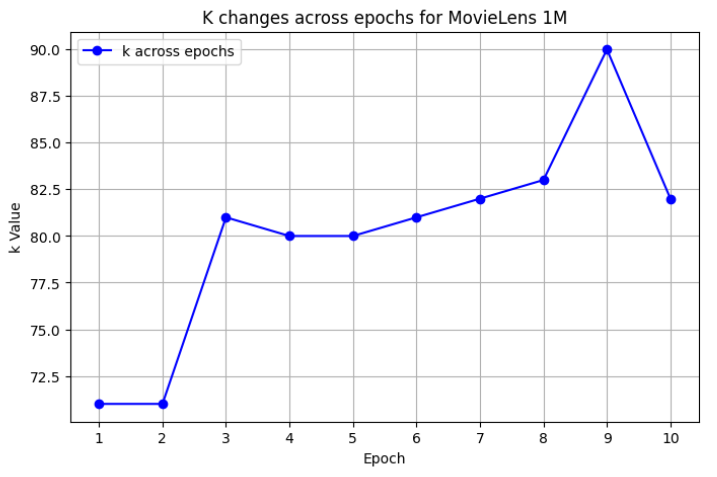
\includegraphics[width=\linewidth]{Figures/chnages_inK_for_1M.png}
		\caption{K changes across epochs for MovieLens 1M}
		\label{fig:k_changes_1M}
	\end{subfigure}
	\caption{Comparison of K changes across epochs for different datasets}
	\label{fig:k_changes}
\end{figure}
the value of K changed dynamically during training, with different behaviors. For the MovieLens 100K dataset, K showed a steady increase across epochs, whereas for the MovieLens 1M dataset, K began at a lower value, experienced fluctuations, peaked, and then stabilized. This indicates that the larger dataset necessitated more adaptive adjustments in retrieval compared to the smaller dataset.\\
Figure~\ref{histo_p} summarizes the performance of our hybrid algorithm compared to the MoL-based approach on the MovieLens 100K and 1M datasets, both tested using a Max Sequence Length of 50, an Embedding Dimension of 128, 2 Attention Heads, a Feedforward Dimension of 128, a Batch Size of 128, and trained for 10 epochs . \\
\begin{figure}[ht]
	\centering
	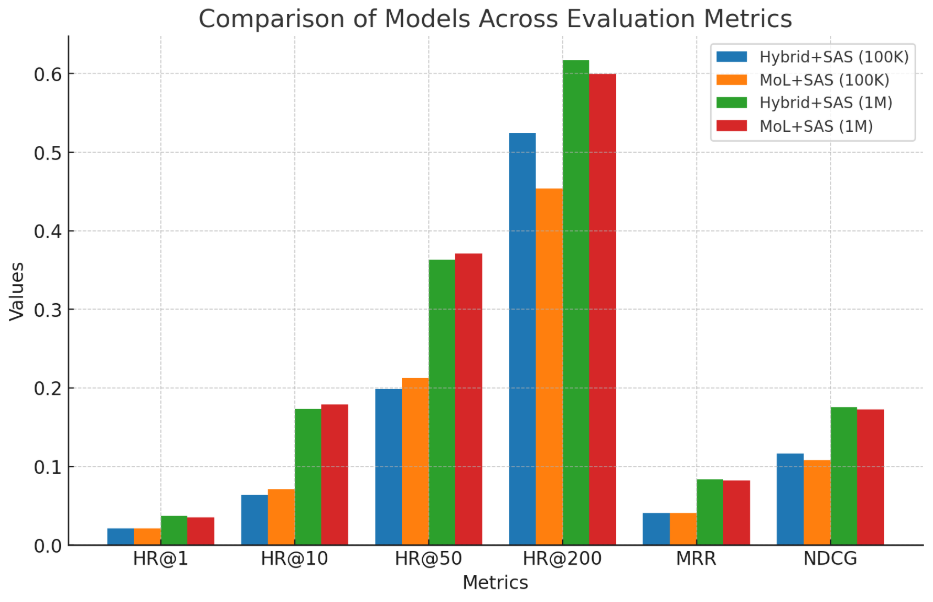
\includegraphics[width=0.7\textwidth]{Figures/HISTOGRAM.png}
	\caption{Comparison of Models Across Evaluation Metrics}\label{histo_p}
\end{figure}
The variations in K help explain the performance differences seen in the fig \ref{histo_p}. The Hybrid+SAS model applied to the MovieLens 1M dataset, which exhibited more dynamic changes in K achieved higher HR@50(0.3631) and HR@200(0.6170) scores, reflecting better long-range recommendation quality. The fluctuations in K in the 1M dataset likely allowed the model to balance exploration and precision, improving its overall ranking performance.

On the other hand, the more gradual K increase in the 100K dataset resulted in relatively lower scores, suggesting that a static or overly conservative 
K selection might limit retrieval effectiveness.

Additionally, the MoL+SAS model achieved better performance than Hybrid+SAS in HR@10 for both datasets. This aligns with the observation that MoL+SAS tended to retrieve fewer but more relevant items at shorter ranking positions. This behavior can be attributed to how K evolved during training?smaller K values in earlier epochs likely enabled MoL+SAS to maintain higher precision at shorter ranks.
These findings highlight the importance of dynamically tuning K based on dataset characteristics to optimize recommendation effectiveness.


The results demonstrate that the Hybrid Exact Top-k algorithm effectively leverages both sequential user behavior and item metadata to improve recommendation quality. The adaptive MoL threshold allows the model to dynamically refine candidate items during training, leading to better performance. The improvements are consistent across both datasets, highlighting the robustness of our approach.\\
%%=============================================%%

\section{Conclusion}

The experimental results demonstrate the effectiveness of our proposed algorithm when applied to SASRec. Through extensive evaluation on the MovieLens-100K and MovieLens-1M datasets, we observe that our method consistently outperforms the baseline models, including SASRec with MOL. Our approach shows improvements in key evaluation metrics, particularly in Hit Rate (HR@k) and Normalized Discounted Cumulative Gain (NDCG@k), indicating better recommendation relevance. Furthermore, the results highlight the importance of hyperparameter tuning, as different configurations significantly impact model performance. 
Overall, the findings confirm that incorporating our algorithm enhances sequential recommendation capabilities, making it a promising approach for future research and real-world applications. Future work will focus on further optimizing the model and testing on additional datasets to validate its generalizability.
